% \pgfplotsset{compat=1.18, width=7cm}

\begin{itemize}
    \item twocolumn
    \item multicols
    \item Minipage
\end{itemize}

\section{Introduction}
\lipsum[1-2]

% \newpage
% \lipsum[1-1]\\

\begin{multicols}{2}[Esta sección del documento esta bien chida.]
    \lipsum[1]
    \myfigure{
        \begin{tikzpicture}
            \begin{axis}[xmin=-2, xmax=2, ymin=-1, ymax=2, axis lines=middle,]
                \addplot[color=black, samples=100]{x^2};
            \end{axis}
        \end{tikzpicture}
        \mycaption{Gráfica cuadrática}
    }
    \lipsum[1]
    \myfigure{
        
\includegraphics[width=0.5\textwidth]{UGTO.png}
        \figcaption{\emph{Im a figure caption}}
    }
    \lipsum[1-2]
    \myfigure{
        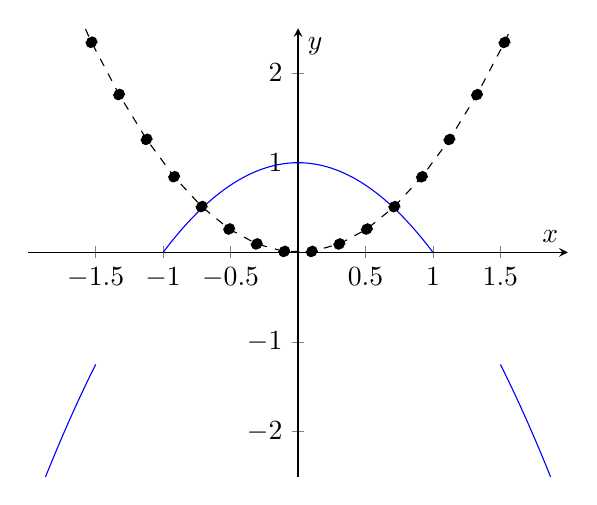
\begin{tikzpicture}
            \begin{axis}[xmin=-2, xmax=2, ymin=-2.5, ymax=2.5, axis lines=middle, xlabel=$x$, ylabel=$y$, title={}, xtick={-1.5, -1, -0.5, 0.5, 1, 1.5}]
                \addplot[color=black, dashed, mark=*, samples=50]{x^2};
                \addplot[color=blue, samples=100, domain=-1:1]{1-x^2};
                \addplot[color=blue, samples=100, domain=-2:-1.5]{1-x^2};
                \addplot[color=blue, samples=100, domain=1.5:2]{1-x^2};
                \end{axis}
        \end{tikzpicture}
        \mycaption{Parabola con $p^+$ y $p^-$ y otra con dominio cortado.}
    }
    \lipsum[1-2]
    \myfigure{
        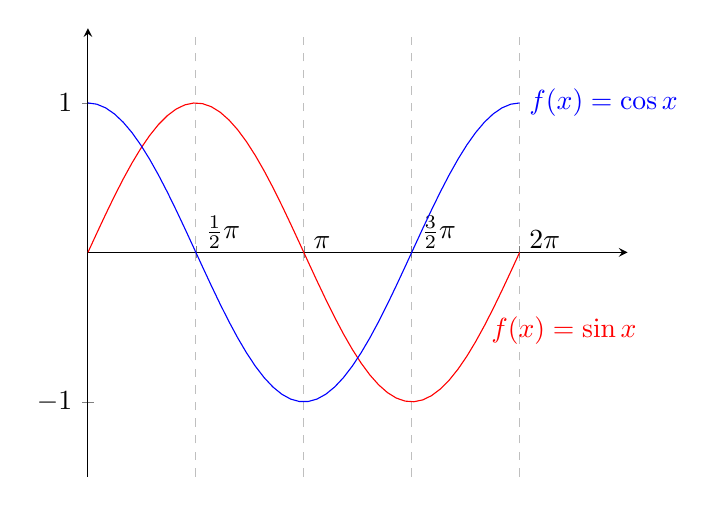
\begin{tikzpicture}
            \begin{axis}[clip=false, xmin=0, xmax=2.5*pi, ymin=-1.5, ymax=1.5, axis lines=middle, xtick={0,pi/2, pi, 3*pi/2, 2*pi}, xticklabels={$0$, $\frac{1}{2}\pi$, $\pi$, $\frac{3}{2}\pi$, $2\pi$},xticklabel style={anchor=south west}, xmajorgrids=true, grid style=dashed]
                \addplot[domain=0:2*pi, color=red, samples=50]{sin(deg(x))}node[right,pos=0.9]{$f(x)=\sin x$};
                \addplot[domain=0:2*pi, color=blue, samples=50]{cos(deg(x))}node[right,pos=1]{$f(x)=\cos x$};
            \end{axis}
        \end{tikzpicture}
        \mycaption{Gráfica Senoidal y Cosenoidal}
    }
\end{multicols}